\documentclass[a4paper, 12pt, garamond]{book}
\usepackage{cours-preambule}
% \graphicspath{{./figures/}}

\usepackage{relsize}

\dominitoc
\faketableofcontents

% \renewcommand{\mtcSfont}{\small\bfseries}
% \renewcommand{\mtcSSfont}{\footnotesize}
\mtcsettitle{minitoc}{}
\mtcsetrules{*}{off}

\setlength{\mtcindent}{-10pt}
\mtcsetoffset{minitoc}{-10pt}

\makeatletter
\renewcommand{\@chapapp}{Fiches -- numéro}
\makeatother

% \toggletrue{student}
% \toggletrue{corrige}
% \renewcommand{\mycol}{black}
% \renewcommand{\mycol}{gray}

\hfuzz=5.002pt

\begin{document}
\setcounter{chapter}{4}

% \settype{book}
% \settype{prof}
% \settype{stud}

\chapter{Python et incertitudes par simulation \textsc{Monte-Carlo}}

% \vspace*{\fill}

\begin{tcn}(appl)<ctc>"somm"'t'{Sommaire}
	\let\item\olditem
	\vspace{-15pt}
	\minitoc
	\vspace{-25pt}
\end{tcn}

\begin{tcn}(appl)<ctb>"how"'t'{Capacités exigibles}
  \begin{itemize}[label=\rcheck]
      \item Simuler, à l'aide d’un langage de programmation ou d’un tableur, un
            processus aléatoire permettant de caractériser la variabilité de la
            valeur d’une grandeur composée.
      \item Simuler, à l'aide d’un langage de programmation ou d’un tableur, un
            processus aléatoire de variation des valeurs expérimentales de
            l'une des grandeurs – simulation \textsc{Monte-Carlo} – pour évaluer
            l'incertitude sur les paramètres du modèle.
  \end{itemize}
\end{tcn}

% \vspace*{\fill}
% \newpage

\section{Survivre en \texttt{Python}}
\subsection{Les bases}
\subsubsection{Calcul et affichage basiques}
\begin{tcb}(code)<lfnt>{Code}
  \inputpygments[numbers=left,xleftmargin=10pt]{python}{F05_python_base-1.py}
\end{tcb}

\subsubsection{Fonctions basiques}
\begin{tcb}[breakable](code)<lfnt>{Code}
  % \inputpygments[fontsize=\relsize{-2}]{python}{F05_python_base-2.py}
  \small
  \inputpygments[numbers=left,xleftmargin=10pt]{python}{F05_python_base-2.py}
\end{tcb}

\subsection{Gestion de données}
\subsubsection{Listes}
\begin{tcb}(code)<lfnt>{Code}
  \inputpygments[numbers=left,xleftmargin=10pt]{python}{F05_python_data-1.py}
\end{tcb}

\subsubsection{Tableaux et \texttt{numpy}}
\begin{tcb}(code)<lfnt>{Code}
  \inputpygments[numbers=left,xleftmargin=10pt]{python}{F05_python_data-2.py}
\end{tcb}

\subsection{Automatisation}
% \vspace{-10pt}
\subsubsection{Fonctions personnelles}
\vspace{-10pt}
\begin{tcb}[breakable](code)<lfnt>{Code}
  \inputpygments[numbers=left,xleftmargin=10pt]{python}{F05_python_auto-1.py}
\end{tcb}

\vspace{-25pt}
\subsubsection{Boucles \texttt{for}}
\begin{tcb}(code)<lfnt>{Code}
  \inputpygments[numbers=left,xleftmargin=10pt]{python}{F05_python_auto-2.py}
\end{tcb}

\vspace{-15pt}
\subsection{Tracé de graphiques}
\subsubsection{Minimal (Figure~\ref{fig:mini})}
\begin{tcb}(code)<lfnt>{Code}
  \inputpygments[numbers=left,xleftmargin=10pt]{python}{F05_python_plot-1.py}
\end{tcb}

\noindent
\begin{minipage}[t]{.48\linewidth}
	~
	\begin{center}
		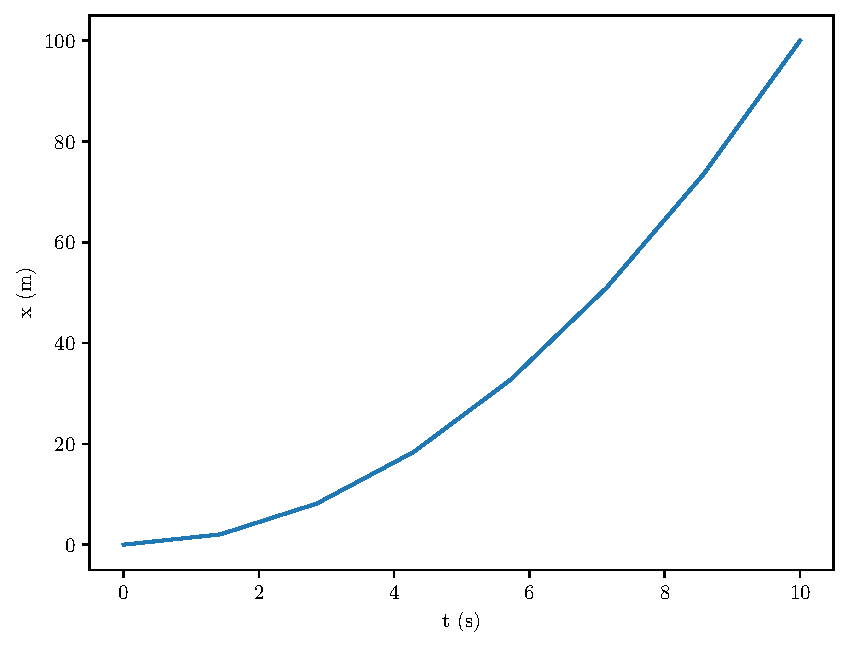
\includegraphics[width=\linewidth]{figures/python_plt-1}
		\captionof{figure}{Figure minimale.}
		\label{fig:mini}
	\end{center}
\end{minipage}
\hfill
\begin{minipage}[t]{.48\linewidth}
	~
	\begin{center}
		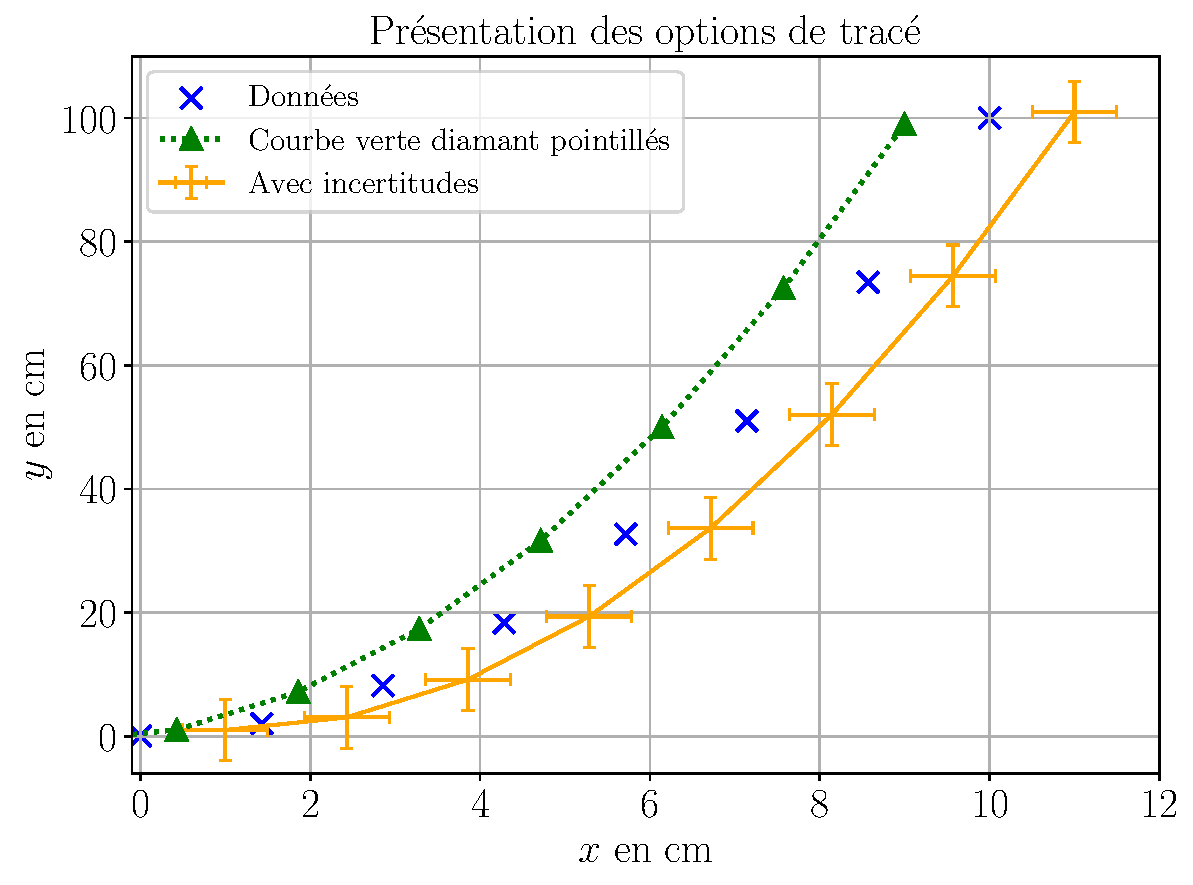
\includegraphics[width=\linewidth]{figures/python_plt-2}
		\captionof{figure}{Figure complexe.}
		\label{fig:cplx}
	\end{center}
\end{minipage}

\subsubsection{Complexe (Figure~\ref{fig:cplx})}
\begin{tcb}[breakable](code)<lfnt>{Code}
  \inputpygments[numbers=left,xleftmargin=10pt]{python}{F05_python_plot-2.py}
\end{tcb}

\section{Simulations \textsc{Monte-Carlo}}
\subsection{Principe}
On dispose généralement de plusieurs jeux de données pour
lesquels on a des incertitudes de mesure, et on veut calculer $z$ qui dépend de
ces données mais d'une manière complexe\ftn{Comprendre~: pas donnée dans la fiche
	\texttt{Mesures et incertitudes}}. On peut alors réaliser une simulation.

En effet, connaissant l'intervalle d'existence des mesures, on peut prendre
aléatoirement d'autres valeurs possibles pour les mesures, et faire toute une
série de calculs avec des valeurs légèrement modifiées. On pourra alors
finalement prendre la moyenne des valeurs calculées et leur écart-type pour
avoir la propagation des incertitudes~!

\begin{tcb}(ror){Cœur de la simulation}
	Finalement, le cœur de la simulation revient (presque) à réaliser une estimation
	d'incertitude de type A sur les valeurs calculées~!
\end{tcb}

\subsection{Application~: mesure d'une distance focale}
On peut mesurer la focale d'une lentille convergente par la méthode de
\textsc{Bessel}~:
\[
	\boxed{f' = \frac{D^{2}-d^{2}}{4D}}
\]
avec $d$ la plage de positions de la lentille qui garde une image nette sur
l'écran, et $D$ la distance objet-écran. S'il est possible de faire le calcul
analytique ici, il peut être plus rapide de réaliser une propagation des
incertitudes des valeurs $d$ et $D$ sur la valeur calculée de $f'$.

Pour cela,
\begin{itemize}[label=$\diamond$, leftmargin=10pt]
	\item On note les valeurs extrêmes de $d$ dans une liste \texttt{d\_xtr}~;
	\item On note les valeurs extrêmes de $D$ dans une liste \texttt{D\_xtr}~;
	\item On créé une liste \texttt{liste\_f} vide qui accueillera les valeurs de
	      $f'$ calculées~;
	\item On fixe $N \gtrsim \num{e4}$ le nombre de simulations~;
	\item Pour $i$ allant de 0 à $N-1$~:
	      \begin{itemize}[label=$\triangleright$, leftmargin=10pt]
		      \item On tire aléatoirement une valeur de $d$ dans l'intervalle
		            \texttt{D\_d}~;
		      \item On tire aléatoirement une valeur de $D$ dans l'intervalle
		            \texttt{D\_D}~;
		      \item On calcule $f'$ avec ces données \textbf{simulées}~;
		      \item On ajoute cette valeur simulée à la liste des valeurs de $f'$.
	      \end{itemize}
	\item On calcule alors la valeur moyenne des $f'$, qui sera la valeur la plus
	      probable, et l'écart-type de la liste des $f'$, qui sera son
	      incertitude-type.
\end{itemize}
\texttt{np.random.uniform(min, max)} est la fonction \texttt{Python} qui permet
de tirer aléatoirement une valeur entre \texttt{min} et \texttt{max}. Ainsi, en
\texttt{Python}~:
\begin{python}
d = 12               # cm
Delta_d = 0.1        # cm
d_xtr = [11.9, 12.1] # cm
D = 50               # cm
Delta_D = 0.5        # cm
D_xtr = [49.5, 50.5] # cm

N = 100000
liste_f = []
for i in range(0, N):
d_simu = np.random.uniform(d_xtr[0], d_xtr[1])
D_simu = np.random.uniform(D_xtr[0], D_xtr[1])
f_simu = D_simu/4 - d_simu**2/(4*D_simu)
liste_f.append(f_simu)

fmoy = np.mean(liste_f)
uf = np.std(liste_f, ddof=1)
print(f'f = {fmoy:.2f} +- {uf:.2f}')
\end{python}

\subsection{Application~: régression linéaire}
Prenons l'exemple de la régression linéaire~:
\[
	y = ax+b
\]
On a mesuré $x$ et $y$, et on obtient $a$ et $b$ avec \texttt{np.polyfit(x, y,
	1)}. Mais ce calcul ne donne pas l'incertitude sur $a$ et $b$. Les deux valeurs
étant interdépendantes, on n'a pas d'expression analytique pour les
déterminer~: on va donc les simuler.

Chaque valeur de $x$ est comprise dans un certain intervalle $x \pm \Delta_x$,
et de même pour $y$. Plutôt que de prendre la valeur centrale et de calculer $a$
et $b$ avec ces valeurs, on peut essayer de calculer $a$ et $b$ pour des valeurs
de $x$ et de $y$ légèrement modifiées. On va donc réaliser un grand nombre de
régressions linéaires en modifiant les valeurs de $x$ et $y$, et on prendra la
moyenne des $a$ et $b$ comme étant la valeur centrale et leur écart-type pour
leur incertitude.

\subsection{En pratique}
\begin{itemize}[label=$\diamond$, leftmargin=10pt]
	\item On détermine les demi-largeurs $\Delta_x$ et $\Delta_y$. Si ce sont des
        incertitudes-types, on aura $\Delta_x = u(x)\sqrt{3}$. Sinon, c'est la
        demi-largeur de la plage des mesures valables.
	\item On fixe un nombre $N$ très grand.
	\item On créé des listes vides \texttt{liste\_a} et \texttt{liste\_b} pour y
	      stocker les futures valeurs des $a$ et des $b$ calculés.
	\item Pour chaque $i$ compris entre $0$ et $N-1$~:
	      \begin{itemize}[label=$\triangleright$]
		      \item on prend \texttt{x\_simu} dans l'intervalle $[x-\Delta_x,
					            x+\Delta_x]$~;
		      \item on prend \texttt{y\_simu} dans l'intervalle $[y-\Delta_y,
					            y+\Delta_y]$~;
		      \item on calcule \texttt{a\_simu} et \texttt{b\_simu} avec ces valeurs
		            simulées~;
		      \item on les stocke dans \texttt{liste\_a} et \texttt{liste\_b}.
	      \end{itemize}
	\item On a alors $N$ valeurs de $a$ et de $b$~: les valeurs les plus probables
	      sont les moyennes, et leurs incertitudes-types sont les les écarts-types des
	      listes de $a$ et de $b$.
\end{itemize}

Ainsi, en \texttt{Python}~:
\begin{python}
x = np.array([0,1,2,3,4, 5,6,7,8,9,10])
ux = 0.1*np.ones(len(x))   # incertitude de 0.1 sur chaque valeur

y = np.array([2.20,2.00,1.60,1.55,1.16, 1.00,0.95,0.60,0.36,0.36,0.18])
uy = 0.12*np.ones(len(y))  # incertitude de 0.12 sur chaque valeur

Delta_x = ux*np.sqrt(3)    # demi-largeur x
Delta_y = uy*np.sqrt(3)    # demi-largeur y

N = 10000                  # nombre de régressions à effectuer

liste_a, liste_b = [], []  # création des listes vides pour stocker les valeurs
for i in range(N):
x_simu = x + np.random.uniform(-Delta_x, Delta_x)
y_simu = y + np.random.uniform(-Delta_y, Delta_y)

a_simu, b_simu = np.polyfit(x_simu, y_simu, 1)

liste_a.append(a_simu)
liste_b.append(b_simu)

a_moy, b_moy = np.mean(liste_a), np.mean(liste_b)
ua, ub = np.std(liste_a, ddof=1), np.std(liste_b, ddof=1)

print(f'Coef.directeur = {a_moy:.3e} +- {ua:.3e}')
print(f"Ordonnée à l'origine = {b_moy:.3e} +- {ub:.3e}")
\end{python}

\end{document}
